\documentclass[10pt, a4paper, oneside]{article}
\usepackage{fancyhdr}
\usepackage{lastpage}
\usepackage{graphicx}
\usepackage{pdfpages}
\usepackage[margin=1 in]{geometry}

\graphicspath{ {./img/} }

\title{Shipwars Online}
\author{Group 4\\Klaus Reche Riisom - Klrii14@student.sdu.dk - Eksam Nr. 65376824\\
Rasmus Lassen - Ralas14@student.sdu.dk - Eksam Nr. 411187\\
Martin Fabricius - Mfabr14@student.sdk.dk - Eksam Nr. 64754120\\
Martin Slusarczyk Hubel - mahub14@student.sdu.dk - Eksam Nr. 411321\\
Niels Bonde Nielsen - Nieni14@student.sdu.dk - Eksam Nr. 409455}
\date{December 2015, 3. Semester}


\fancypagestyle{derp}{%
\fancyhf{}
\fancyhead[L]{University of Southern Denmark\\3. semester, Software Engineering}
\fancyhead[R]{Project group 4\\11/9 - 2015}
\fancyfoot[C]{Page \thepage\ of }
\renewcommand{\headrulewidth}{0.2pt}
\renewcommand{\footrulewidth}{0.2pt}
}


\begin{document}
\pagestyle{empty}
\maketitle

\newpage
\pagestyle{derp}

\renewcommand\thesection{\roman{section}}
\renewcommand\thesubsection{\thesection.\roman{subsection}}
\setcounter{page}{1}
\pagenumbering{arabic}

\tableofcontents
\newpage
\listoffigures
\newpage
\input{tex/abstract}
\newpage

\section{Preface}
The following report is the documentation that describes how the software was developed and why the group made the choices it did. It has been written in connection to with the bachelor degree in software engineering on the University of Southern Denmark - 3. Semester. The project has been developed as a part of the course “Design of software systems in a global context”. The group would like to thank Claudio Giovanni Mattera for the help and advice giving during this project.
\\
\\
This report should be read chronologically to ensure the full understanding of the subject and the choices made by the group.
\\
\\
By signing below here, the group members confirm that they all have been active in and contributed to, the project.
\\
\\
\\

\noindent\rule{10cm}{0.4pt}                                                                  Date: 18/12/2015.
\\
\\
\\
\noindent\rule{10cm}{0.4pt}                                                                 Date: 18/12/2015.
\\
\\
\\
\noindent\rule{10cm}{0.4pt}                                                                 Date: 18/12/2015.
\\
\\
\\
\noindent\rule{10cm}{0.4pt}                                                                 Date: 18/12/2015.
\\
\\
\\
\noindent\rule{10cm}{0.4pt}                                                                 Date: 18/12/2015.
\\
\\
\\
\noindent\rule{10cm}{0.4pt}                                                                 Date: 18/12/2015.

\newpage

\chapter{Editorial}
\begin{figure}[h]
\centering
\centerline{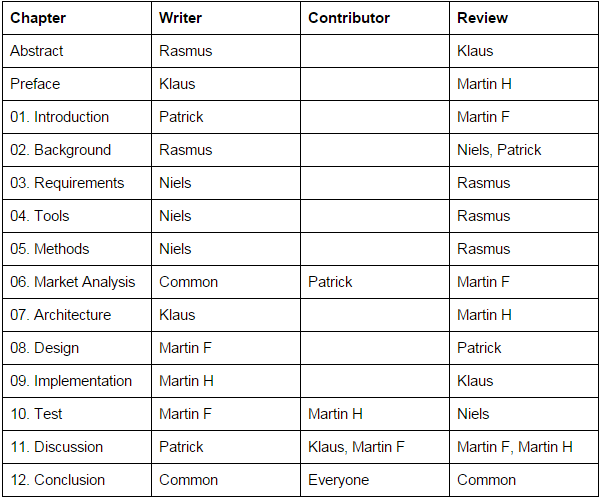
\includegraphics[scale=0.96]{Editorial} }
\end{figure}

\newpage

\renewcommand\thesection{\arabic{section}}
\renewcommand\thesubsection{\thesection.\arabic{subsection}}
%\pagenumbering{arabic}


\section{Project Introduction}

	This semester’s project definition was more open than the last
	 two semester projects. We only had to make a distributed system.
	  So we were free choose a topic, as long as it included a client,
		 a server and a database, which were all connected to make an application.
	\\
	\\
	The project handbook actually gave a case where we could develop
	 a system that would help newly started firms make their way into
	  China’s market for production. We decided that we wanted to
		make something else, so we started brainstorming about what
		 each of us wanted to make, then we all came to the agreement
		  of making a game. After that we brainstormed again, this time
			 about what kind of game we wanted to make. It ended up with
			  the classic board game “Battleship” that we would make into
				 a digital version called “Shipwars”. The game fit the criteria
				 perfectly for the requirements we needed. It could have a client
				 that connects to a server that also have a connection to a database
				  where user data is stored. The game would also fulfil our courses
					requirements on this semester project with things like encryption on
					 user data and a market analysis for the cross culture
					  management course. With this game we would eliminate
						the need for being together in the same room when playing, and
						 instead open the possibility to play against people across
						 the globe.
	\\
When we agreed upon the game and its topic, we had to write a project
formulation, and decided to write about the background of board games.
	\\
	\subsection{Project Formulation}

	As board games are rooted in the physical world, board games are limited
	 to the people who can play against each other locally. In order for
	 physical board games to connect a larger player-base that can play anywhere
	  anytime, the Internet may be necessary in order to make it available
		 worldwide. This creates certain problems and here are the ones the
		  group will focus on solving:
	\begin{itemize}
		\item How to digitize a board game?
		\item How to connect multiple people via the Internet?
		\item How to differentiate between the players?
	\end{itemize}

\newpage

\chapter{Background}

This section will touch upon the subjects of the varying popularity between
 board games and video games, and try to explain some of the main reasons why
 they are varying.\newline

The concept of playing games has existed for a very long time, but its meaning
 has changed through time. Just a decade or two ago computers were not as
 normal to possess as they are now, and by “playing games” people usually
 referred to some game involving physical activity or playing with physical
  objects. Chess is a good example of this and it is probably one of the
  oldest games that are still being played today.
Families would usually gather around the table at late evenings and have a
good time together before bedtime.\newline

Due to technological advancement, computers now have a fixed spot in the
 homes of almost any family living in modern societies, and the term “games”
 has reached a much broader meaning. Whereas people who grew up in the
  60 - 70’s would most likely “play games” in shape of physical board
  games like chess, play cards or something similar, today’s generation
  has a much wider range of opportunities, such as computers and gaming
   consoles. And it seems to be the trend to play games through computers
    and consoles, because as an article from telegraph.co.uk states it with
     a survey:\newline

"The survey suggested that while 73 per cent of parents remembered regularly
 playing board games as children, only 44 per cent of the children polled said
 they do so now"\footnote{http://www.telegraph.co.uk/men/relationships/fatherhood/11696224/Card-games-and-board-games-are-dying-out-and-its-no-great-loss.html}\newline

The reason for the board games' gradually decreased popularity, besides
 the technological progress, may also be connected with the games themselves.
  As board games are games involving physical objects, their value of
   experience is thereby limited. In order to play board games the participants
   have to be physically present at the same place as the games take place in
   the physical world. Video games, on the other hand, takes place in the
   digital realm and thus they offer another level of experience. But the
   thing that makes video games truly special, and has been a core factor
   of video games’ success in recent years is the concept of online
    multiplayer.\newline

An online multiplayer means you have the opportunity to play against other
players from all around the world. This means that when people play games
online on a multiplayer game, they very often play with or against people
they have never met or seen before. This concept is often called
“the separation of space and time” and it is one of the major by-products
 of technological advancement; you basically chat and interact with players,
  even if they are sitting on the other side of the planet, and the responses
   are instant.
Since board games are physical, they are subject to break sooner or later or
at least miss a piece of the game thus making the game impossible to play.
 Video games does not have this problem since they have no physical shape.
 All they take to play is an installation and they do not age the same
 way. \newline

If board games, or just the games, are to survive in a time with video games
gaining popularity, the games must be digitized so it will be possible to play
 on the devices most people use these days: The computer, console or
 smartphone. \newline

Ultimately this means it is no longer a board game when it has been digitized.
 But the game is the same - it has the same rules. But the way it is played is
  just different.\newline

\newpage

\section{Requirements}

This chapter is used to explain the thoughts on the requirements that
 were made for the project. This covers analyzing what is involved in creating
  a game. The scope for the project will be covered and finally the use cases
   for the project will be introduced and explained.

\subsection{Game Development Analysis}

The following analysis covers games and gaming split into two parts.
The first part covers the concept of games. The second part covers the
issues with game development.\\\\
The concept of a game can be seen as a goal-oriented experience,
where a group of various activities is played out by one or more players.
These activities are to provide a form of enjoyment or pleasure through
 competition either with oneself or others. In order to keep the game
  consistent rules are imposed onto the game.
In this way, a game employs interactivity and participation of a user,
referred to as a player. The player is put into a scenario with rules and
 goals, where the scenario could be either a reference to or abstraction of
  a realistic situation. The player either gets a goal provided by the game,
   or the player creates their own goal. The goal must be completed to “win”
    the game. Getting into a position of inability or failure to complete the
     goal results in “losing” the game.\\\\
Developing a game can bring certain issues. One of those issues is
 presentation. If the player cannot effectively interact with or understand
  what they are seeing or reading, their experience may not lead to enjoyment.
   Another issue is interaction. Without the proper options to complete the
    required goals, the player may not be able to fulfill the goal. This can
     again lead to an undesirable experience. A third issue is efficiency. If
      the game is unplayable because of inefficiencies, or stability issues,
       the player may not even want to play the game.

\subsection{Scope}

The game will contain an online access functionality that utilizes
 a client-server structure connecting with a database, as the game will
  make use of user accounts for the client, it will be necessary to encrypt
   all user account information. The group choose to use .NET as the
    framework for developing the client-server structure, since C\# is used
     for programming. \\
The game will be very limited in graphics and aesthetics, since the
 focus of the development is on the technical aspects. The group have
  therefore chosen to limit the game to 2D graphics with very simple
   turn-based functionality, and make our own version of the classic
    board game Battleship. The group decided to make the game multiplayer
     to fulfill the distributed system part of the project.

\subsubsection{The Board Game}

The board game “Battleships” is build up around a basic turn based game,
with a grid size of 10x10. Before the game starts each player chooses the
 spot for each of their five ships. Each round a player chooses a coordinate
  to which he attacks from his side to the opponent side. If it is a hit, the
   opponent places a red pin in the boat that is a hit, and the same does the
    player who fired. If it is a miss, the firing player must place a white
     pin in the coordinate to show that the shot did not hit. Each player
      then have five ships in varying sizes up to five pins long. When a
       ship has been sunk the opponent must say what kind of ship that is
        down. When one of the players have lowered all the opponent's
         ships, they win.

\subsubsection{The Computer Game}

The computer game will incorporate the board game’s functionality,
 and make most of it automated. In the first round each player places
  their ships location on the boards’ grid. In the next rounds until a
   player has won, the players will switch turns when a tile has been
    chosen. During the current player’s turn, that player will be shown
     a larger version of the opponent’s grid with their ships locations
      hidden. The player will then choose a tile on the grid to reveal
       whether or not there is a ship. If there is a ship, the tile will
        be marked in red, if not the tile will be marked in gray. A player
         has won when all of the opponent's ships have been fully revealed.

\subsection{Use Case Diagram}

The use cases made for the project were assigned a category in order to
 differentiate between them. The categories were assigned after where the
  use cases’ functionality were most prevalent. UC means the code made for
   the client layer, US for server and lastly UD for database.

\subsubsection{Actors}

\textbf{Player}: Will be interacting with the system though the client.\\
\textbf{Client}: Software part that is responsible for the GUI and the connection
 to the Server. \\
\textbf{Server}: All the software logic will be located here\\
\textbf{Database}: Here the data will be stored.

\begin{figure}[h]
\centering
\includegraphics[scale=0.5]{usecase}
\caption{Usecase diagram}
\end{figure}
\clearpage

\subsection{Use Case Priority}

In order to prioritize our use cases, the group focused on three factors:
 First the amount we were going to learn from realizing the functionality
  involved. Second how important the use case is for fulfilling the
   requirement of the project. Lastly how important the functionality
    is for the final product, if some function is required in another
     use case as well. The more of these criteria, the use case fulfills,
      the higher it is prioritized.

\begin{figure}[h]
\centering
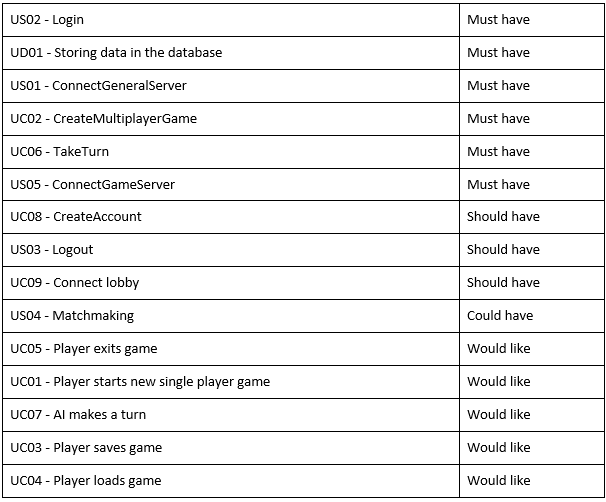
\includegraphics[scale=0.7]{Priority}
\caption{Usecase priority}
\end{figure}
\newpage
\subsection{Use Case Description}
The report will be focusing on 2 use cases to show an idea of the thoughts
 behind the process.

First one will be the creation of a game\\

\begin{figure}[h]
\centering
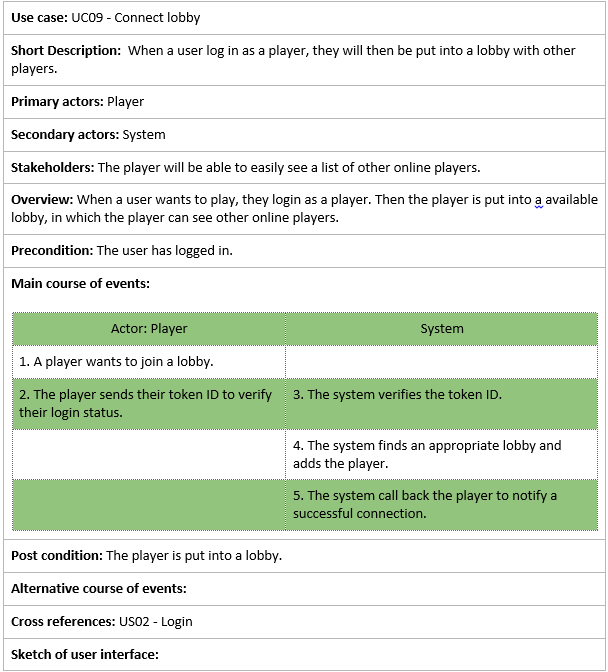
\includegraphics[scale=0.8]{usecon}
\caption{Usecase description for UC09}
\end{figure}
\clearpage

Second one is when the game is started and the player makes a turn.\\

\begin{figure}[h]
\centering
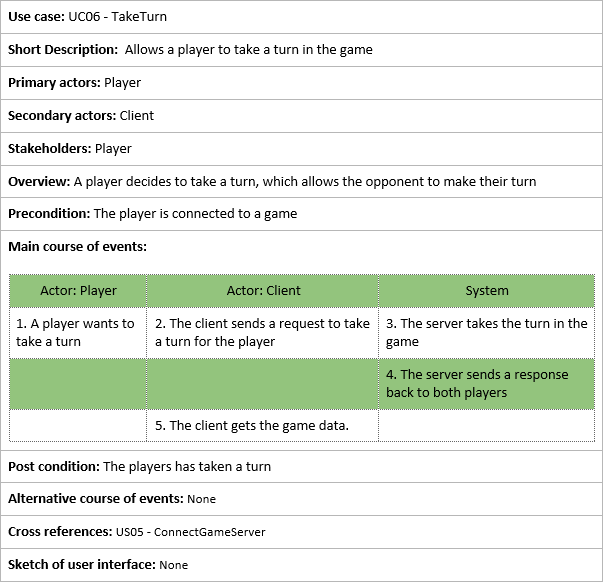
\includegraphics[scale=0.8]{usetak}
\caption{Usecase description for UC06}
\end{figure}
The remaning can be found in the appendix \ref{appendix:useCase_specification}

\newpage

\section{Tools}

This chapter will go through all the software
used in the project.

\subsection{Development tools}

These are the software used directly for developing
 the software

\subsubsection{Git}

Git is a widely used version control system,
 used by project groups to collaborate as a
  team. When used it creates a repository,
  which makes a history over the changes to
  make it possible to rewind to an earlier
  stage. This was used as the version control
  system for the project.
\subsubsection{Github}

Github is a git server hosting service. It
 makes a server host a git repository available
 for a team to work on. Most of the hosted
 projects are made available to the public
 as an open source project for others to
  explore and give feedback on. This was used
as the host service for our git repository.

\subsubsection{Visual Studio}

Visual Studio is one of the most used IDE’s for
 programing a broad range of programming
languages. It was used in this project to
 make all the C# code the final product
  consists of.

\subsection{Project Management}

These were the software used for managing the task present in the project.

\subsubsection{Trello}

Trello is a time management website used to create a virtual to-do list. When
 a board is created for the team all the members will be able to contribute to
  the board. It was used as the tool to manage our project’s development cycles
   and divide the different use cases equally between the groups.

\subsection{Modelling Tool}

This where the tools used to create artifacts for the project.

\subsubsection{Draw.io}

Draw.io is an online diagram tool able to collaborate with different cloud
 services. The diagrams created here can be shared with the team, allowing
  multiple people to edit

\subsection{Text Editor}

This were the tool used for creating the documentation created during
 the project.

\subsubsection{Latex}

 LaTeX is a document modeling language. It allows the user to design
  a document from scratch in plain text. When the document is done it compiles
   the plain text into the finished text file. This is the tool used to create
    the final report as it provides a high level of control over the fine
     details like layout, design and formatting.

\subsubsection{Google Docs, Google Drive and Microsoft Word}

These were used to make and share documents in the group during the
 development, in a less formal way. Google Docs was our primary text
  editor, where Word was used for assignments.

\newpage

\section{Methods}

In this section the methods used in the project will be explained and why they were used.

\subsection{Unified Process}

We used UP as a guideline for the project as a whole, which means
that Scrumban was our main structure for the project, and during the
start of the project the inception phase of UP was used when we created
 the inception document.

\subsection{Scrumban}

This is an agile method for creating a product. It is a hybrid
between Scrum and Kanban, utilizing the best of both methods. It
 combines the sprint iteration style from scrum with the bucket list
  and whiteboard planning style of Kanban. It works by putting all the
   requirements for the project onto sticky notes. This then becomes the
    backlog for work, and when a scrum sprint starts the requirement is
     evaluated by its importance. This helps to prioritize the task for a
      given sprint. There is also a limit on how many requirements that can
       be worked on at a given sprint, which will help to make sure that
        resources are not spend unnecessarily and the tasks get done.

\newpage
\chapter{Market Analysis}
	In the course CCM, the group had to make a market analysis which
   investigates the possibilities of selling the software on the global
   market. To find out if it is viable and how to go about it. A study
    on a fictional company, that the group made up, was done and also a
     study of a chosen market’s culture was done for the use to potentially
      further development of our software.
	\\
	\section{Going international or not?}
	Reasons for going international:
	\begin{itemize}
		\item Bigger Market
		\begin{itemize}
			\item Thanks to the fact that our product is developed in an
       international language, it is accessible for a broad audience
		\end{itemize}
		\item Bigger Audience
		\begin{itemize}
			\item A simple fact is that there are not many big game development
       companies in our little country. So if we want to become a part of
        a bigger company, we will need to get seen by as many as possible
		\end{itemize}
	\end{itemize}
	Reason not to go international:
	\begin{itemize}
		\item Difference in cultures may cause conflicts/disagreements
		\begin{itemize}
			\item Different countries may have different views on what a good game
       looks like. If we should choose to distribute to a country that
        dislikes our product, the country may give us a bad image based
         on their views
		\end{itemize}
	\end{itemize}
	\begin{itemize}
		\item Need for bigger hardware specs
			\begin{itemize}
				\item If we distribute our game for a bigger market, the hardware
         specs will need to be higher as there will be more users and
          longer between the player
			\end{itemize}
	\end{itemize}
	\begin{itemize}
		\item Need for broader company staff across countries
	\end{itemize}
	\begin{itemize}
	\item 	If we would go international there’s a high possibility the resources
   needed to maintain the company will exceed our current staff’s limits.
    Therefore, we would have to hire staff in different countries, which
    can be both good and bad. The bad thing could be that it would make
    it more difficult or complicated to maintain an overview of the company
     and the progress altogether. And eventual conflicts will be difficult
     to appropriately handle.
		 \end{itemize}
	\\
	\section{SWOT Analysis}
	In here we look at our fictional company’s goals and strengths, and how
   our product will fare on the market.
	\\
	\subsection{Mission and Goals}
	Our small game company, Small Dinghy Software, consist of six students
   and is focused and determined to make a game for the international market,
    and to make a profit from the sales of the game. We don’t plan to make a
     living of the sales, only to make a profit. The focus will be on the
     western market, but will still be accessible on a global scale. This
     will be done using the Steam platform from Valve Corporation, which
     in turn will be a huge benefit for future customers and handling of
     taxation.
	\\
	\subsection{Eternal Environment}
	\textbf{Legal protection and rights}
	\\
	Our game Shipwars Online, which is based on the classic board game
   “Battleships”, could not use that name, since it was licensed by the
   company who made the movie “Battleships”. This was the reason for naming
    the game Shipwars Online instead. We could in turn license the name
     “Shipwars” as a franchise, to ensure that our game will not be mistaken
      for another game with the same name.
	\\
	\\
	\textbf{Trade restrictions}
	\\
	Since we currently only plan to use the Steam platform as our sales
  platform, we will be limited to the users of Steam as our potential
  customers, which is not a bad thing, since Steam has a huge user/customer
  base of approximately 6 million people online on the service every day.
	\\
	\begin{figure}[h]
	\centerline{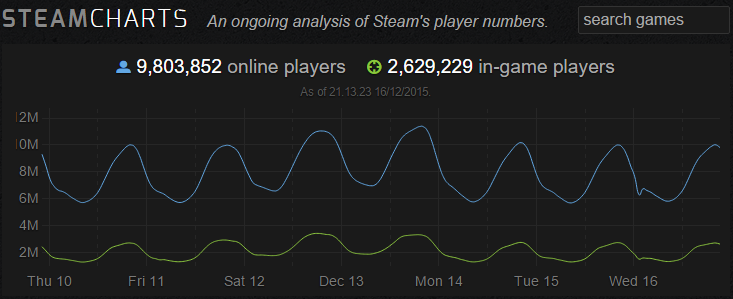
\includegraphics[scale=0.63]{SteamCharts}}
	\caption{Steam chart of users playing}
	\end{figure}
	\\
	\textbf{Shifting Production \& Consumption}
	\\
	Competing software products emerging on Steam can change the balance of
   consumption and sale of Shipwars Online. Clones could emerge that try to
    take a share of the market. Sales on Steam can push more people to buy
    the product if wanted by the developer. In terms of production, it is
    basically nothing, as the product only exists as an intangible virtual
     product.
	\\
	\\
	\textbf{Strengths}
	The strengths in our company is the game itself. With an internationally
  known game that has a similar style as the original board game
  “Battleships”, we hope that the memory of the board game will attract
  the players to our online game. The game will be bought for a one-time
   fee, and after be free for the user to play. Our company focuses on
    keeping the game interesting and fun for the gamers around the world.
     With the skilled employees, we aim to keep the game professional and
     up to date.
The highest cost in our firm will be the server maintenance, that have to
withstand the pressure of a high amount of players.
	\\
	\\
	\textbf{Weaknesses}
	The marketing for our company is low budget. As we are a new player
  on the market, we need to keep cost down, but also distribute our game
   out to the public. Therefore, online advertisement on different sites
    are what we can afford for now. The competitions are the board game
     itself, and as it stands we have the upper hand, that is mostly because
     of the growing industry online, where the board games are beginning to
     lose market share. On the technical front we are not the most developed.
	\\
	\\
	\textbf{Opportunities}
	The game is online and therefore it fits with the emerging trends of online
   games. Access to an international market allows a potential large
    player-base growth if the marketing and choice of platform is just right.
	\\
	\\
	\textbf{Threats}
	Most of the threats to our product comes from the fact that our company
   is not big, so we don’t have access to a big security network. An example
   would be that we don’t have much claim on our game in terms of copyright
   and access to lawyers if someone violates it.  Also we have to consider
    the copyrights of the company who first developed the “Battleship” board
     game and make sure we have an agreement with them before releasing our
     online version.
	\\
	\\
	As the company’s products focus on software the international market would
   be the ideal candidate. Software can be deployed across most of the world,
    as it can be distributed wirelessly and wired through the Internet.
    Software can be targeted to any specific country if needed, since the
    code is not set in stone.
	\\
	\section{Strategy for going international}
	Entering an overseas market in relation to Denmark requires looking into
   physical and virtual platforms situated in these locations. Physical
    platforms allow software to be resold through export to various
     brick-and-mortar businesses around the world. Virtual platforms allow
      software to be sold through either third-party licensing or through
       direct sales in a home-brewed platform.
	\\
	\\
	In America, the virtual platform Steam is available as a software
   distributor, mostly focusing on games. Steam allows a software
   organisation to deploy and sell their software requiring no exclusivity.
    What Steam gets from this deal is a cut on the sale. Steam only applies
     to desktop (Windows, OSX, Linux), so other platforms would be needed in
      order to supplement other directions such as mobile
      apps (eg. App Store and Google Play Store).
	\\
	\\
	The company chose the licensing strategy. This was done because it would
   let the company keep control and ownership of the product. It also opens
    up for the possibility that the company can expand the product to other
     international markets. Another reason to keep control of the game is so
      that the company can improve and expand the game.
	\\
	\\
	Licensing also allows a small, if not non-existent, transport cost. Any
   transport cost would be with network bandwidth. However, with a third-party
    licensing platform, such as Steam, this cost is shifted onto the
     platform owner, instead of the developer.
	\\
	\\
	The company chose the Steam platform because Steam offer a lot of help
   to small companies and individual developers who wish to release games
    but does not know the intricacies of licensing policy.
	\\
	\\
	We have also tried to check if different cultures would react differently
   to our game. There was not much information on the subject, other than
   some countries can ban your game if they find it offensive. Because our
   game is a remake of the old board game, the likelihood of the game being
    banned is minimal. Also the age group for our customers, would most
    likely be in the age regime of nearly all ages. This is again because
     it is a board game, and can be played with everybody as soon you know
     the rules to the game, and it will be fairly simple to play.

\newpage

\section{Software Architecture}
In this section the group will describe how it used software architecture
 in the project, the different choices the group made to ensure that the
  system runs according to the specifications, defined by the group, and
   how the work was planned, executed and then possibly changed so it would
    work better. It will also describe the structure of the system and how
    the system has been distributed.
\\
\subsection{Architecture}
As told earlier in the report the group has chosen to make an online version
of the game Battleship. With this in mind the group generated several
requirements in the form of use cases, these use cases are listed in the
Requirements chapter and in that section it is also shown how they were
prioritized by the group. The requirements were split into groups based
on what part of the system they dealt with, and prioritized using MoSCoW
as explained in the section.
\\
\subsubsection{Client-Server}
The main goal of the project was to make a distributed system. This the group
accomplished by separating the system into three distinct components, the
client, the server and the database. These three components run on different
 computers, the client and server are two standalone applications.
\\
\\
A distributed system is a collection of independent computers. Each computer
has its own processor and memory. This allows each computer to work
independently of each other. In order to utilise the resources of each
computer, the computers are connected via various communication architectures.
 Examples of such a communication architecture include buses and wireless
  connections.\footnote{Silberschatz et al. 2010, p. 719}
\\
\\
One way to set up the computers is through a client-server architecture. A
computer acts as a server, whilst other computers act as clients or other
servers, such as a database server. The benefits of this setup are resource
sharing, computation partitioning, connection-reliability and communication
capabilities.\footnote{Silberschatz et al. 2010, pp. 720-721}
\\
\\
Since the group decided to make a game, a client-server pattern was the
obvious choice, especially when the system had to be distributed, the client
was separated so it could run as a stand-alone application. The pattern also
makes the server accessible from different places at once, and allows the
player to play against each other online.
\\
\\
In relation to games, distributed systems allows multiple player clients to
connect to a centralised server, working as an interface for all client
requests. Examples of client requests include verifying account information,
updating the game state, or communicating with other player clients.
\\
\\
One of the major problems with the client-server architecture is the strain
on the server bandwidth. In MMORPGs such as World of Warcraft or EVE Online
thousands of concurrent player clients connect to a server. This is possible
by utilising multiple servers in their own distributed system. This allows
the servers to distribute the computation load to multiple
servers.\footnote{Winn et al. 2013, pp. 3-4}
\\
\subsubsection{Layer}
The group chose a layered approach to ensure maintainability and to make it
so that the game easily could be separated into its components. The group
chose to make it a 3-layer architecture pattern where the game was split
into 3 parts: (1) Presentation layer, (2) Business layer and (3) Data layer.
\\
\\
\textbf{Presentation layer:} : In this layer the interface is located.
It is here that the group developed the GUI and made use of facades.
This was to ensure maintainability since it means that the GUI or any
other part is relatively easy to change out, as there is no direct
connection between the layers. As long as the facades remain the same
the system does not care how the GUI looks or how it works.
\\
\\
\textbf{Business layer:} Here is where all the logic of the game is
located. This is where the game functionality lies and how it does it
is defined. How the connection between the server and the clients worked
 will be explained in the Service-Oriented sub section.
\\
\\
\textbf{Data layer:} This is where the database is located, again
accessible by a facade to make maintainability easy and separate concerns.
 This is a separate component in this system as the database is is not in
 the same place as the server or any of the clients. The database is where
  all the reusable information is stored. Information like user-information,
  usernames, e-mails, passwords etc. is stored in the database. The data is
   sent over a secure connection and the information is encrypted to make sure
    that none of the information given by the users can be stolen.
\\
\subsubsection{Service-Oriented}
The server follows a service-oriented architecture (SOA), allowing client
 and server to communicate through a common interface.
 The service-orientation works by making interfaces that act as facades
  for logic. As explained earlier this is to ensure that the logic can
   be maintained easily on the server, and easily on the client by developers
    without server knowledge.
\\
\\
The advantages of SOA is distributing a reusable, loosely coupled and
 standardized service, allowing anonymous access from clients, where
  messages can be either synchronous or asynchronous. It is defined by
  a contract and a concrete implementation, where the client uses the
  contract to access the
  implementation.\footnote{Vogel et al. 2011. pp. 206-207}
\\
\subsubsection{Security}
In order for a user to be authorized and authenticated in the game,
they first need to login. This is done using a single sign-on (SSO)
architecture, where a token is created and provided to the client upon
successful login.\footnote{Vogel et al. 2011. p. 220} The server tracks
the session of the token and controls how it is used. The client now does
not need to login again, but simply use the provided token. In this project,
this token can be used to connect to the game service in order to start
 playing against others. This has the advantage of allowing a client to
  use any service that supports the token after logging in. The disadvantage,
   though, is that all services supporting the token need a connection to
   the service verifying the token.
\\
\subsection{View Model}
There are several different architectural view models, but the group decided
to work with the 4+1 architectural view model, as this model revolves around
 the use of use cases, which is a main point of the group’s Scrum/Kanban
 development approach. The model contains six views: (1) Use case view, (2)
  Logical view, (3) Implementation view, (4) Data view, (5) Process view,
  (6) Deployment view. Looking through the project, the group has primarily
   been working with the Logical and Implementation views but have used most
   of them to various degrees. Most of the project have been spent on the
    implementation of the system and during that time, the group mostly look
    at it from the Implementation view. During the planning of the project
     it was mostly looked at from the Logical view, though many of the
     requirements were defined as use cases it is clear that the Use case
     view was used. Moreover since the system is distributed it has also
     been looked at from the Process view.
\\
\\
\textbf{Use case view:}
\\
This is the basis for the 4+1 view model, it is from this view that all the
 other views make their architectural decisions. To show all the use cases
 and how they interact with each other and the user, the group has made a use
  case diagram, this diagram has already been shown in the Requirements chapter.
\\
\\
\textbf{Logical view:}
\\
This view looks at how the use cases will be implemented. It is used to get
 an overview of the the code is going to look, how the different classes will
  work together, and what methods and attributes the classes will contain. The
   group made a class diagram for each package in the project. They can be
    seen in the appendix \ref{appendix:class_diagrams}
\\
\\
\textbf{Data view:}
\\
This view is used to describe the data models and how they interact with the
 system. Since the group used ADO.NET to make the database, an entity model
 was created and from this, the database was automatically created. The entity
  model can be seen and is explained in the chapter Implementation.
\\
\\
\textbf{Process view:}
\\
This view focuses on the behaviour of the system while it is running, and
how the different use cases cause different classes to interact with each
other and how. To show this the group developed some sequence diagrams, but
 after the first few sprints it was decided that they were not used enough
 to warrant the time spend on creating them. But those that have been made can be seen in appendix \ref{appendix:sequence_diagrams}.
\\
\\
\textbf{Deployment view:}
\\
This view describes how the static artefacts are deployed in the physical
world. This the group has shown by making a deployment diagram, which shows
how the system is separated into three parts, and how they connect to each
other. Here is the deployment diagram shown:
\begin{figure}
\centerline{\includegraphics[scale=0.65]{Deployment} }
\caption{Deployment Diagram}
\end{figure}

\newpage
\input{tex/design}
\newpage
\input{tex/implementation}
\newpage
\input{tex/test}
\newpage
\chapter{Discussion}
	In this chapter we will briefly go over our accomplishments in the project
   period and what we think could have been done differently. There will also
    be a short description on how we used the courses of the semester in the
     project.
	\\
	\\
	We started out with the idea of making an online multiplayer turn based
   game which had the functionality of battling against each other. Through
    the semester we have expanded the project with the knowledge we learned
     from our courses.
	\\
	\section{Did we reach our personal goals?}
	We did manage to develop a simple online game where multiple people can play
   against each other. We would have liked to get more graphical in our game,
    but this was not in the requirements so we made a simple GUI instead of
    going after an advanced one, so we could get more of our use cases
     implemented.
	\\
	\\
One of the major things we wanted to learn while making this game, was how
 to use the programming language C\#, and how it was different from Java.
 We all learned to varying degrees to code in C\#. This is a great benefit
 for our future, as it is a language that is often used and therefore very
 a useful skill to have.
	\\
	\section{Did we reach the goal for our semester?}
	In terms of distribution and networking, we successfully implemented a
  distributed product, allowing connections between client and server, and
   server and database.
We tried our best to integrate the different courses into our project. Our
 plan was to implement encryption between the client and server, but due to
  time constraints we couldn’t. So now we only have a token system that
   verifies the user connecting to the server, but the password is send as
    a plain text file over the network, instead of being encrypted. We
    integrated CCM in the form of our market analysis. OPN was integrated
     as our code, and was fulfilled since we managed to create a distributed
     system. Finally DES was integrated as a guideline for our architecture
     where we split the code up into three main layers: Client, Server and
     Database. It made more sense to the group and made it so we had a good
      view of the code.
	\\
	\section{Did we follow SOLID and GRASP?}
	We did not quite follow the guidelines from SOLID and some of the patterns
   from GRASP, which we should change if we were to continue working on the
    game. The reason we lost sight of using them, might be because most of
    us had not used C\#,  WCF, or WPF before. So our focus was instead to
    try and implement a working distributed system.
	\\
	\section{Could we sell the game as it is now?}
	If we want to sell the game ourselves then no, but we would be able to
  sell the game if we fixed the things mentioned above. It is hard to say
   if we could sell the game on the international market, since our market
    analysis does not go into great detail how the international market
     would respond to such a game. If we were to go on the international
     market, it would be wise to make a new analysis that looks into how
     the market would respond and whether or not it would be viable for us
      to do so. This would imply that we would have to maintain the server
       and the cost would have to be covered by the sale of the game. However,
        as our market analysis shows if we use Steam we could reach an
         international audience, but we do not know if it would sell.
	\section{Project Problems}
	During this project there has been some issues that the group have had to
   deal with. One was that the group chose to write the code in C\#, which is
    a programming language that most of the group had not worked with before.
    The reason the group chose to write in C\# was to expand the skillset of
     the group, but it caused the development of code to be slow since the
     group had to learn the differences between Java and C\#. One of these
      differences was that the group was taught how to network in Java and
      that it would be perfect for client-server interaction. Because of that
      the group tried to find C\# equivalents, which WCF was, culminating in
       the use of this in the project.
	\\
	\\
	The distribution of the system is not currently across multiple machines but
   rather only locally. This is due to several issues with compatibility of
   certain technologies and time involved. The provided Linux server can not
    directly use .NET without some intermediary. The mono framework can be
    used to replace .NET, but we did not have time to get this installed, as
    we were still trying to figure out .NET. In terms of the database, the
     provided one used PostgresSQL, which requires additional setup in Visual
      Studio in order to get to work with the ADO.NET entity model framework.
       We did initially work with a PostgresSQL library to create a connection
       to the database and work directly with SQL queries, but it quickly
       became time-consuming. In the end we settled with keeping it locally,
        but still open for change in terms of connectivity.
	\\
	\section{Project successes}
	On the other side there were also some things that the group did very well.
   In this project the group have worked very well together without any
   problems in the group, and everyone have done their share. Also the use
    of Kanban made the development of the software very structured and easy
     to keep an overview on.
	\\
	\\
If there was anything the group should have done differently it might be to
 make sure the entire group had studied more on the new programming language.
  There were a few in the group that had worked with it before, but the rest
  had never touched it. If those that had never touched it had studied it more
   diligently then maybe there would not have been the problem of slow code
    development. Otherwise we should have written either server or client in
    java, and the other in C\#.

\newpage
\input{tex/konklusion}
\newpage

\Chapter{Bibliography}

\section{Printed Works}
\begin{itemize}
	\item Silberschatz, A., \& Galvin, P.B., \& Gagne, G. (2010).
   Operating System Concepts with Java: John Wiley \& Sons. Inc.
   \item Winn, J., \& Bright, T., \& Jensen, C.G., \& Teng, C. (2013). Utilising game server technology on fully distributed architectures for collaborative multi-user CAx applications: Taylor \& Francis Group.
   \item Vogel, O., \& Arnold, I., \& Chughtai, A., \& Kehrer, T. (2011). Software Architecture: Springer
\end{itemize}

\subsection {Online References}
\begin{itemize}
	\item Microsoft 1. Remotable and Nonremotable Objects. Retrieved 16/12/2015, from https://msdn.microsoft.com/library/h8f0y3fc.aspx
	\item Microsoft 2. .NET Framework Remoting Architecture. Retrieved 16/12/2015, from https://msdn.microsoft.com/en-us/library/2e7z38xb.aspx
	\item Microsoft 3. What Is Windows Communication Foundation. Retrieved 16/12/2015, from https://msdn.microsoft.com/en-us/library/ms731082.aspx
	\item Microsoft 4. How to: Create a Duplex Contract. Retrieved 16/12/2015, from https://msdn.microsoft.com/en-us/library/ms731184(v=vs.110).aspx
	\item Microsoft 5. NetNamedPipeBinding Class. Retrieved 16/12/2015, https://msdn.microsoft.com/en-us/library/system.servicemodel.netnamedpipebinding.aspx
	\item Microsoft 6. ThreadPool Class. Retrieved 16/12/2015, https://msdn.microsoft.com/en-us/library/system.threading.threadpool.aspx
	\item Microsoft 7. Dispatcher Class. Retrieved 16/12/2015, https://msdn.microsoft.com/en-us/library/system.windows.threading.dispatcher.aspx
	\item Microsoft 8. Concurrency Management. Retrieved 16/12/2015, https://msdn.microsoft.com/en-us/library/orm-9780596521301-02-08.aspx
	\item Microsoft 9. Types Supported by the Data Contract Serializer. Retrieved 16/12/2015, https://msdn.microsoft.com/en-us/library/ms731923.aspx
	\item Microsoft 10. Using Data Contracts. Retrieved 16/12/2015, https://msdn.microsoft.com/en-us/library/ms733127.aspx
	\item Microsoft 11. Chapter 7: Message and Transport Security. Retrieved 16/12/2015, https://msdn.microsoft.com/en-us/library/ff648863.aspx
	\item Microsoft 12. Building Secure ASP.NET Applications: Authentication, Authorization, and Secure Communication. Retrieved 16/12/2015, https://msdn.microsoft.com/en-us/library/ff649205.aspx
  \item srp.pdf, Retrieved 02/2002, Robert C. Martin:   http://www.objectmentor.com/resources/articles/srp.pdf
  \item ocp.pdf, 01/1996, Robert C. Martin:   http://www.objectmentor.com/resources/articles/ocp.pdf
  \item Principles_and_Patterns.pdf, 01/2000, Robert C. Martin: http://www.objectmentor.com/resources/articles/Principles_and_Patterns.pdf
\end{itemize}

\newpage

\renewcommand\thesection{\alph{section}}
\renewcommand\thesubsection{\thesection.\alph{subsection}}
%\pagenumbering{alph}
\section{Appendix}
\subsection{Class Diagrams}
\label{appendix:class_diagrams}
\begin{figure}[h]
\centerline{\includegraphics[scale=0.36]{ClientProject} }
\caption{Client diagram}
\end{figure}
\newpage
\begin{figure}[h]
\centerline{\includegraphics[scale=0.8]{GameDataProject} }
\caption{Game Data diagram}
\end{figure}
\newpage
\begin{figure}[h]
\centerline{\includegraphics[scale=0.36]{GameProject} }
\caption{Game diagram}
\end{figure}
\newpage
\begin{figure}[h]
\centerline{\includegraphics[scale=0.25]{GameServicesProject} }
\caption{Game Services diagram}
\end{figure}
\newpage
\begin{figure}[h]
\centerline{\includegraphics[scale=0.45]{GeneralServicesProject} }
\caption{General Services diagram}
\end{figure}
\newpage
\begin{figure}[h]
\centerline{\includegraphics[scale=0.43]{SecurityTokenServicesProject} }
\caption{Security Token Services diagram}
\end{figure}
\begin{figure}[h]
\centerline{\includegraphics[scale=0.36]{ServerProject} }
\caption{Server diagram}
\end{figure}
\newpage

\subsection{SOLID}
\label{appendix:SOLID}
There are 5 principles to SOLID:
\\
\\
\textbf{Single Responsibility Principle (SRP)}
\\
 “There should never be more than one reason for a class to change.”\footnote{srp.pdf, 02/2002, Robert C. Martin, page 1}
\\
\\
This principle focus on cohesion, and means that a class should only be assigned one responsibility, by splitting a class that has multiple responsibilities into different classes. This will allow for good maintainability, since if later some requirements changes, that would mean a change in responsibility amongst the classes as well.
\\
\\
\textbf{Open/Closed Principle (OCP)}
\\
"Software entities (classes, modules, functions, etc.) should be open for extension, but closed for modification."\footnote{ocp.pdf, 01/1996, Robert C. Martin, page 1}
\\
\\
The principle means that we should write our software entities to be extended without modifying the code. This will be achieved by abstraction, since it allows us to change what the software entity does, without changing the code.
\\
\\
\textbf{Liskov Substitution Principle (LSP)}
\\
"Subclasses should be substitutable for their base classes."\footnote{Principles\_and\_Patterns.pdf, 01/2000, Robert C. Martin, page 8}
\\
\\
This means that a subclass of the base class should still function properly, even if a derived class of the base class is passed to it. A violation of LSP, will also result in a violation of OCP.\footnote{Principles\_and\_Patterns.pdf, 01/2000, Robert C. Martin, page 12}
\\
\\
\textbf{Interface Segregation Principle (ISP)}
\\
"Many client specific interfaces are better than one general purpose interface."\footnote{Principles\_and\_Patterns.pdf, 01/2000, Robert C. Martin, page 14}
\\
\\
This means that we should create specific interfaces for each client and inherit multiple of them, instead of one class with all the methods a client would need.
This does not mean that every class that has a service, should have a special interface. Clients should instead be categorized by their type, and then create interfaces for each type. Then if different client types need the same method, it should be added to their interface.\footnote{Principles\_and\_Patterns.pdf, 01/2000, Robert C. Martin, page 15}
\\
\\
\textbf{Dependency Inversion Principle (DIP)}
\\
"Depend upon Abstractions. Do not depend upon concretions."\footnote{Principles\_and\_Patterns.pdf, 01/2000, Robert C. Martin, page 12}
\\
This means that every dependency should be on an interface or an abstract class, not a concrete class or function.
\\
\newpage
\subsection{GRASP}
\label{appendix:GRASP}
There are 9 patterns to GRASP\footnote{Applying UML and patterns, Larman 2005}:
\\
\\
\textbf{Controller}
\\
Controller pattern is used to create a non-UI class that can represent more than one use case. An example of this could be create user and delete user which would have a single controller together.
\\
\\
\textbf{Creator}
\\
The creator pattern uses one class to create other classes in cases where the creator monitors or uses the class it creates. It can have the initialization information for the class and passes it on when the class is created.
\\
\\
\textbf{High Cohesion}
\\
High cohesion is a pattern that attempts to keep objects manageable and understandable. This is achieved by breaking programs into smaller classes and subsystems. If the system is a low cohesion the code can be hard to reuse, maintain and averse to change.
\\
\\
\textbf{Indirection}
\\
Indirection pattern is a low coupling pattern. It takes the mediation between two classes and give them to an intermediate object. An example of this is the introduction of a controller for meditation between data and its representation.
\\
\\
\textbf{Information Expert}
\\
Information expert is a principle is used to delegate responsibilities. Responsibilities includes methods, computed files, and so on. A common use is to look what information is needed to complete it and then determine where that information is stored.
\\
\\
\textbf{Low Coupling}
\\
Low coupling is how much an object have knowledge, relies on and connected to other elements. The low coupling pattern is used to assign the responsibilities to support: low dependency, higher reuse potential and change in one class does not have a big impact on other classes.
\\
\\
\textbf{Polymorphism}
\\
If it is needed to handle alternatives based on a type, polymorphism should be used. An example of this would be if there was two types Dog and Cat, they are both just alternatives to each other. Instead polymorphism should be used, which results in creating a common type Animal, where Dog and Cat are its alternatives by extending or implementing depending on the type.
\\
\\
\textbf{Protected Variations}
\\
This pattern is similar to the Open/Closed principle of SOLID, and should be used when
a change/variation in the software will or would cause the software to be unstable. This is done by using an interface and polymorphism to wrap the old code instead of modifying it directly.
\\
\\
\textbf{Pure Fabrication}
\\
If the Information Expert fails the Pure Fabrication pattern steps in. This is done by creating a class that does not represent the domain concepts. In other words, if the responsibility assigned by the Information Expert does not meet the high cohesion, create a separate class and assign responsibility to it, so that it results in high cohesion.

\newpage
\subsection {UseCase Specification}
\label{appendix:useCase_specification}
\multido{\i=1+1}{10}{%
  \begin{frame}
    \centering
    \includegraphics[width=.9\linewidth]{usecase\i}
  \end{frame}
\newpage
}
\newpage

\subsection{Collaboration Agreement}
\textbf{Academic goals}
\begin{itemize}
	\item Reach an understanding in the subject of ‘Software System Design in a Global Context’.
	\item Ability to utilise the experience from last semester’s project.
\end{itemize}
\textbf{Social goals}
\begin{itemize}
	\item Reach an acceptable collaboration environment.
	\item Sustain a reasonable atmosphere in the group to avoid problems between group members.
	\begin{itemize}
		\item If any problems should occur, they should be solved swiftly and completely to avoid further issues.
	\end{itemize}
	\item Problems are solved through direct contact with the person in question.
	\item If a problem still remains unsolved after contact with the person in question, contact should be established with the advisor Claudio Giovanni Mattera (cgim@mmmi.sdu.dk) and 	supervisor Ulrik Pagh Schultz (ups@mmmi.sdu.dk)
\end{itemize}
\textbf{Level of ambition}
\\
The group's level of ambition is that all the members of the group perform their best to reach the highest of results.
\\
\\
\textbf{Organisational and work norms}
\begin{itemize}
	\item In the event of major group disagreements a democratic voting system will be used, ensuring all voices are heard and compromises are made.
	\item The group meets every friday at 10 a.m., unless otherwise announced.
	\item If meeting attendance is not possible, it should be announced to the rest of the group as quickly as possible.
	\item Each group member is responsible for the content of the final report and other deliverables.
	\item If a break is needed, the group should be notified beforehand.
	\item If an assigned deliverable cannot be done in time, the group should be contacted beforehand, allowing other group members to be able to help if possible.
\end{itemize}
\textbf{Group Norms}
\begin{itemize}
	\item Discussions must be kept at a reasonable level.
	\item Each group member cleans up after themselves.
	\item If attendance is not possible and no announcement has been made thereof, the matter may be brought up with the advisor or supervisor depending on the severity.
\end{itemize}
\newpage
\subsection{Advisor Agreement}
The advisor has the responsibility to help the group in the right direction, but the responsibility of the group work and learning is entirely on the group and its members. All group members are expected to attend advisor meetings.
\\
\\
An agenda of subjects for discussion will be prepared and sent to the advisor at least a work day before a meeting. This agenda will be read by the advisor before the meeting. This meeting will be expected to take place once a week if requested by the group. Any cancellations of the meeting must occur a day before the meeting.
\\
\\
Other inquiries including deliverables and other material sent to the advisor is read and sent back with comments in a reasonable timeframe.

\subsection{Sequence Diagrams}
\label{appendix:sequence_diagrams}
\begin{figure}[h]
\centerline{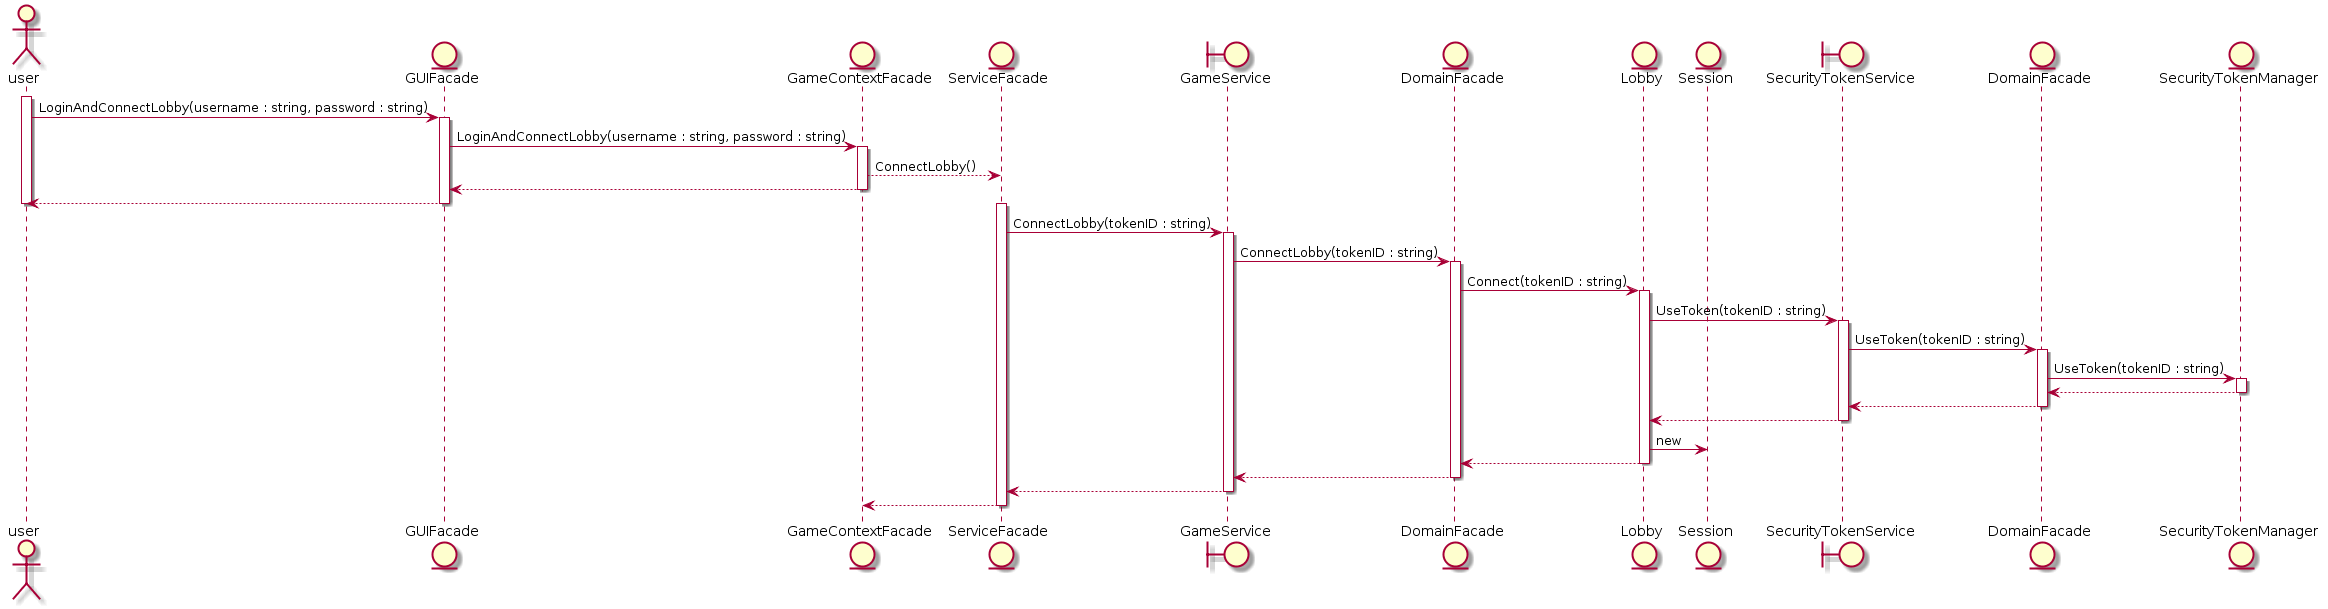
\includegraphics[scale=0.2, angle= 90]{Sequence1} }
\caption{Connect to Lobby Sequence Diagram}
\end{figure}
\newpage
\begin{figure}[h]
\centerline{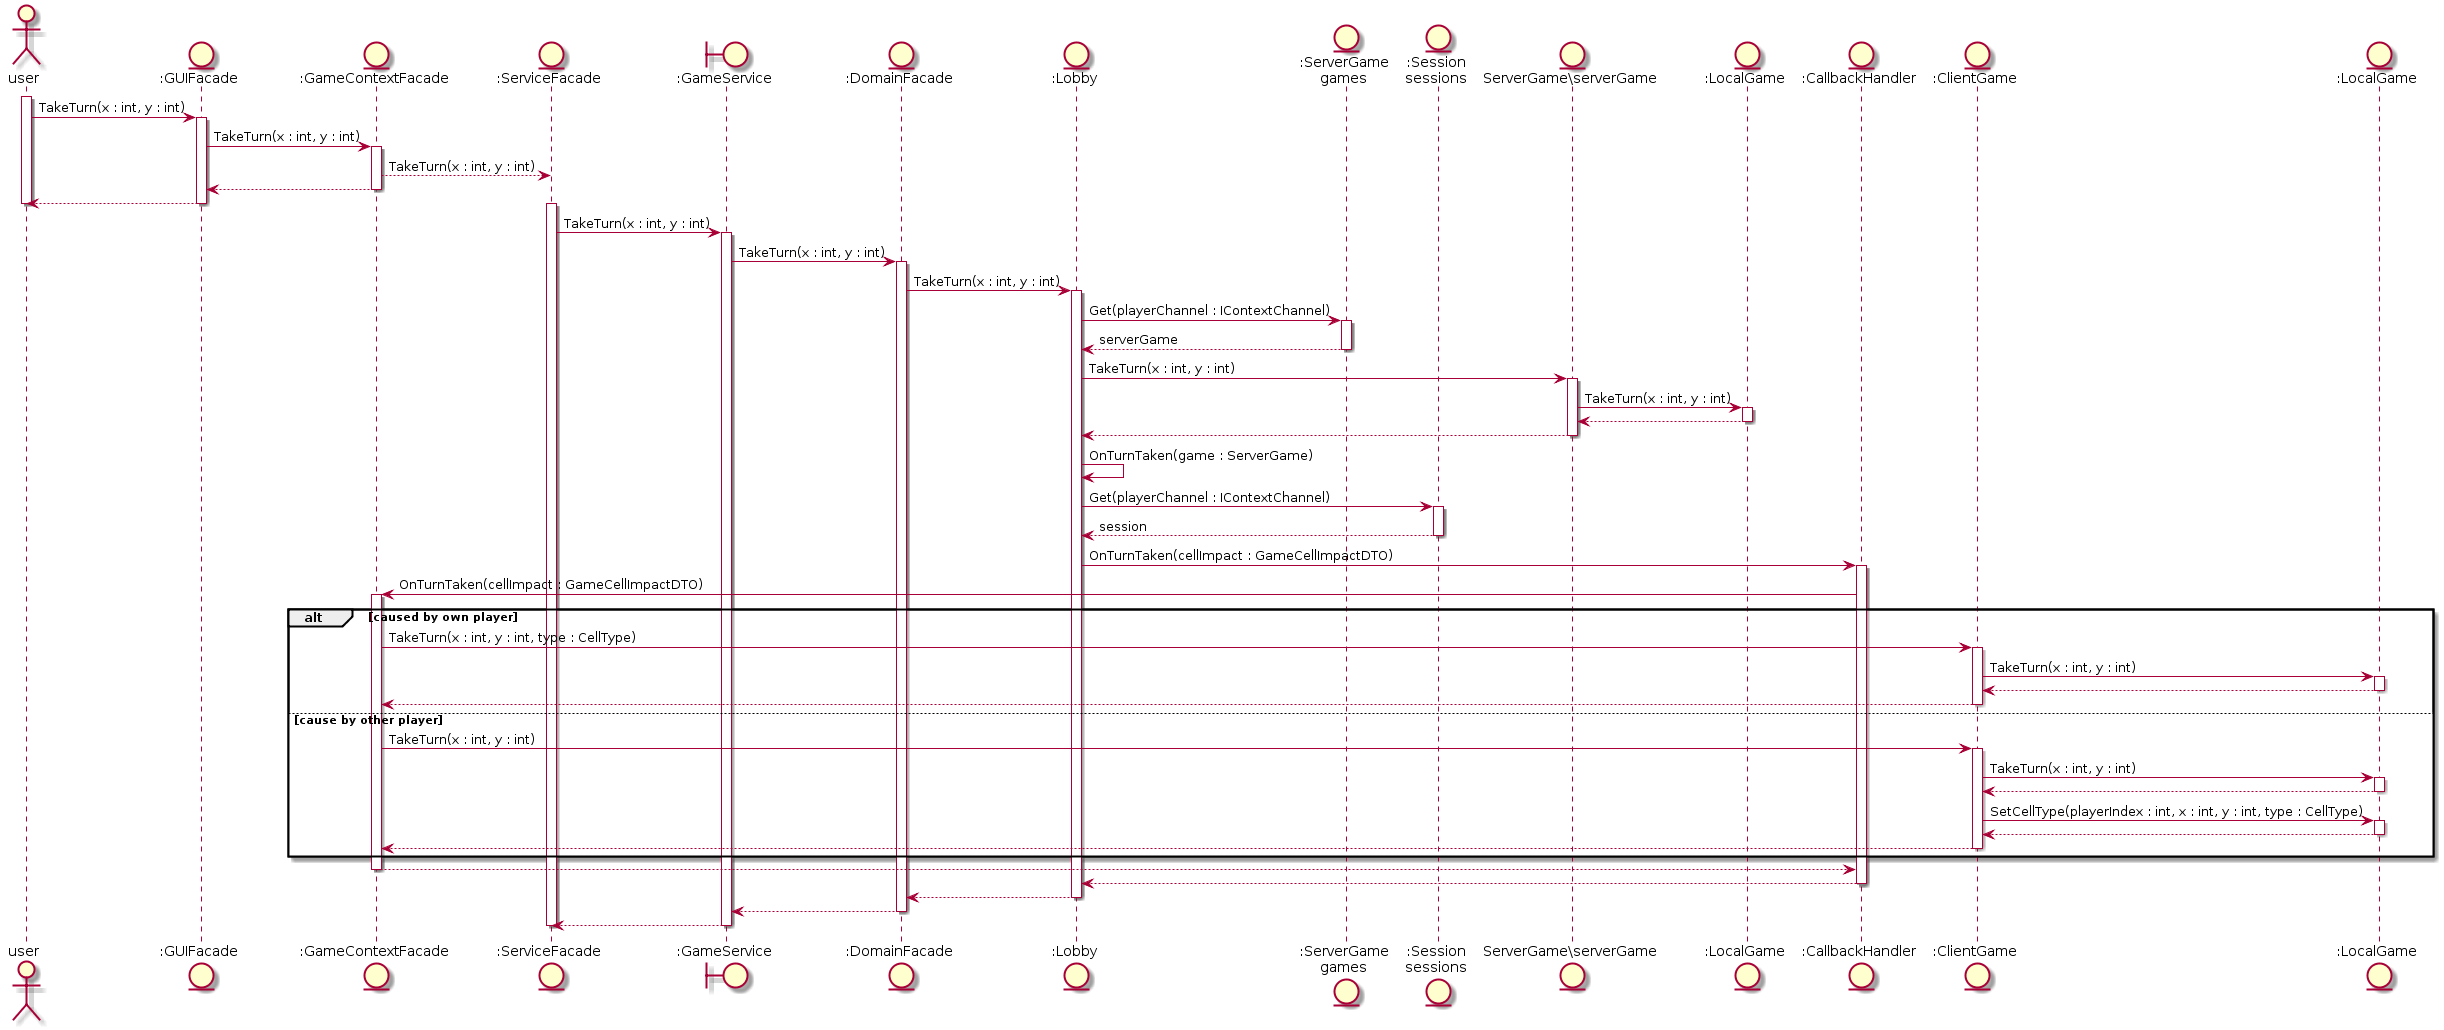
\includegraphics[scale=0.2, angle=90]{Sequence2} }
\caption{Take Turn Sequence Diagram}
\end{figure}

\newpage
%\pagenumbering{arabic}
\end{document}
